\documentclass{article}
\usepackage{qilin}
\tikzstyle{process} = [rectangle, rounded corners, minimum width=1.5cm, minimum height=0.5cm,align=center, draw=black, fill=gray!30, auto]
\title{AER210: Fluid Mechanics Demonstrations}
\author{QiLin Xue}
\date{Fall 2021}
\usepackage{mathrsfs}
\usetikzlibrary{arrows}
\begin{document}

\maketitle
\section{Flow Visualization}
\textit{Note:} I left out the straight-wall diffuser content as it is only an application of flow visualization techniques, and is (probably) not important for the lab. I'm also lazy.

One way of visualizing flow is to use an open surface water channel. A stream of water can be created in a controlled manner and hydrogen bubbles (or dye) can be injected to see the flow in action.
\begin{center}
    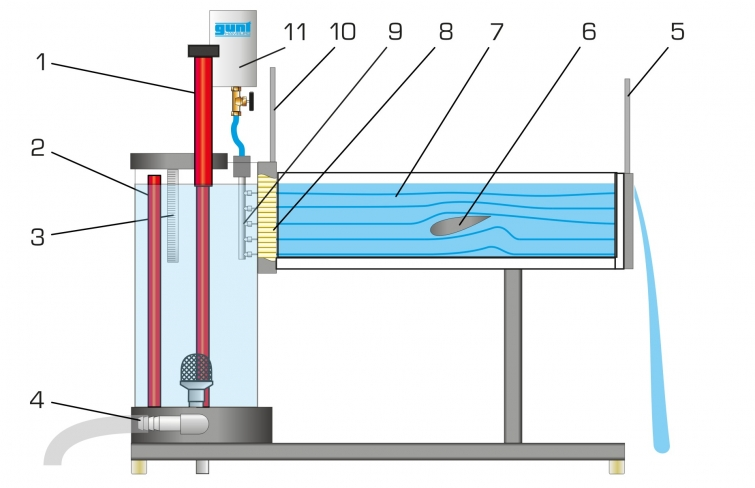
\includegraphics[width=0.4\linewidth]{visual.jpg}
\end{center}
\subsection{Pathlines, Streaklines, Timeline, Streamlines}
We introduce a few definitions: 
\begin{itemize}
    \item \textbf{Pathline:} The trajectory of some fluid element (i.e. the path that a bubble traces out)
    \item \textbf{Streakline:} The instantaneous loci of all fluid elements that pass through a given fixed point. Dye steadily injected into the fluid at a fixed point extends along a streakline.
    \begin{itemize}
        \item In steady state, this is equivalent to the path line.
    \end{itemize}
    \item \textbf{Timeline:} The instantaneous location of a flow of elements at a prescribed location. This is most useful if it is perpendicular to flow, as it allows us to understand the velocity profile.
    \item \textbf{Streamline:} The curve that is instantaneously tangent to the velocity vector of the flow. If the velocity is a function of time, then the shape of the streamlines may vary from instant to instant.
\end{itemize}
For example, consider unsteady flow past an oscillating plate, we can show the differences: 
\begin{center}
    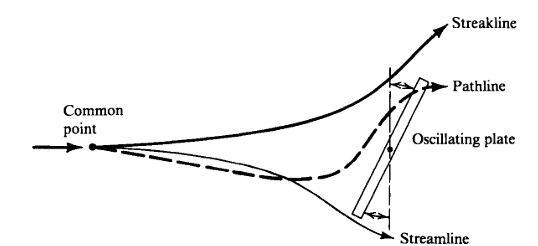
\includegraphics[width=0.5\linewidth]{lines.png}
\end{center}
Specifically, these are all different in a \textbf{transient flow,} which is when the velocity field depends on time. 
\end{document}